% =============================================================================
%  portopt : guide d'utilisation
%  Compilation : cd docs && latexmk -xelatex user_guide.tex
% =============================================================================
\documentclass[11pt,a4paper]{article}

\usepackage{polyglossia}
\setdefaultlanguage{french}
\usepackage{amsmath,amssymb,mathtools}
\usepackage[math-style=ISO,bold-style=ISO]{unicode-math}
\setmainfont{Latin Modern Roman}[SmallCapsFont={Latin Modern Roman Caps}]
\setmathfont{Latin Modern Math}
\setsansfont{space-grotesk-400.ttf}[
  Path=../portopt/fonts/, BoldFont=space-grotesk-600.ttf, Scale=0.95,
  SmallCapsFont=space-grotesk-400.ttf, BoldFeatures={SmallCapsFont=space-grotesk-600.ttf}]
\setmonofont{space-mono-400.ttf}[Path=../portopt/fonts/, Scale=0.86, BoldFont=space-mono-400.ttf]
\newfontfamily\headfont{space-grotesk-600.ttf}[Path=../portopt/fonts/]
\usepackage[autostyle]{csquotes}

\usepackage[a4paper,margin=2.5cm,headheight=14pt]{geometry}
\usepackage{microtype}
\usepackage{xcolor}
\definecolor{accent}{HTML}{2A78D6}
\definecolor{accentsoft}{HTML}{F2F7FD}
\definecolor{warm}{HTML}{EB6834}
\definecolor{warmsoft}{HTML}{FDF3EE}
\definecolor{outbg}{HTML}{F6F6F4}
\definecolor{ink}{HTML}{0B0B0B}
\definecolor{ink2}{HTML}{52514E}
\definecolor{rule}{HTML}{E4E3DF}

\usepackage{graphicx}
\graphicspath{{figures/}}
\usepackage[font=small,labelfont={sf,bf},labelsep=period,skip=6pt]{caption}
\usepackage{booktabs,tabularx,array,longtable}
\usepackage[section]{placeins}
\usepackage{enumitem}
\setlist{itemsep=2pt,topsep=4pt,leftmargin=*}
\usepackage{fancyhdr}
\usepackage{titlesec}
\usepackage[most]{tcolorbox}
\usepackage{listings}
\usepackage{tikz}
\usetikzlibrary{positioning,arrows.meta}
\usepackage[hidelinks]{hyperref}
\hypersetup{colorlinks=true,linkcolor=accent,urlcolor=accent,
  pdftitle={portopt : guide d'utilisation},pdfauthor={Jean Philippe N'DRI}}

\titleformat{\section}{\headfont\Large\color{ink}}{\color{accent}\thesection}{0.8em}{}
\titleformat{\subsection}{\headfont\large\color{ink}}{\color{accent}\thesubsection}{0.7em}{}
\titleformat{\subsubsection}{\headfont\normalsize\color{ink}}{}{0em}{}
\titlespacing*{\section}{0pt}{2.2ex plus .5ex}{1.2ex}
\titlespacing*{\subsection}{0pt}{1.8ex plus .4ex}{0.9ex}
\titlespacing*{\subsubsection}{0pt}{1.4ex plus .3ex}{0.5ex}
\setcounter{secnumdepth}{2}
\setcounter{tocdepth}{1}

\pagestyle{fancy}
\fancyhf{}
\renewcommand{\headrulewidth}{0.4pt}
\renewcommand{\headrule}{\color{rule}\hrule height\headrulewidth}
\fancyhead[L]{\sffamily\footnotesize\color{ink2}portopt \textperiodcentered{} Guide d'utilisation}
\fancyhead[R]{\sffamily\footnotesize\color{ink2}\nouppercase{\leftmark}}
\fancyfoot[C]{\sffamily\footnotesize\color{ink2}\thepage}
\renewcommand{\sectionmark}[1]{\markboth{\thesection\quad #1}{}}

\tcbset{pbox/.style={enhanced,breakable,boxrule=0pt,arc=2pt,outer arc=2pt,
  left=10pt,right=10pt,top=6pt,bottom=6pt,before skip=10pt,after skip=10pt,
  fonttitle=\sffamily\bfseries\small,coltitle=ink,
  attach title to upper={\par\smallskip},fontupper=\small\raggedright}}
\newtcolorbox{attention}{pbox,colback=warmsoft,borderline west={2.5pt}{0pt}{warm},title={Attention}}
\newtcolorbox{note}{pbox,colback=accentsoft,borderline west={2.5pt}{0pt}{accent},title={À savoir}}

\lstdefinestyle{py}{basicstyle=\ttfamily\small,columns=fullflexible,keepspaces=true,
  backgroundcolor=\color{accentsoft},frame=none,xleftmargin=8pt,xrightmargin=8pt,
  aboveskip=8pt,belowskip=4pt,commentstyle=\color{ink2},keywordstyle=\color{accent},
  stringstyle=\color{warm},language=Python,showstringspaces=false,upquote=true}
\lstdefinestyle{out}{basicstyle=\ttfamily\footnotesize\color{ink2},columns=fullflexible,
  keepspaces=true,backgroundcolor=\color{outbg},frame=none,xleftmargin=8pt,xrightmargin=8pt,
  aboveskip=0pt,belowskip=8pt,language={},upquote=true}
\lstdefinestyle{sh}{basicstyle=\ttfamily\small,columns=fullflexible,keepspaces=true,
  backgroundcolor=\color{accentsoft},frame=none,xleftmargin=8pt,xrightmargin=8pt,
  aboveskip=8pt,belowskip=8pt,language=bash,upquote=true,commentstyle=\color{ink2}}
\lstnewenvironment{python}{\lstset{style=py}}{}
\lstnewenvironment{pyout}{\lstset{style=out}}{}
\lstnewenvironment{shell}{\lstset{style=sh}}{}

\newcommand{\py}[1]{{\ttfamily\hyphenchar\font=-1 \detokenize{#1}}}
\newcommand{\pct}{\,\%}
\newcommand{\fig}[3][\linewidth]{%
  \begin{figure}[htbp]\centering\includegraphics[width=#1]{#2}\caption{#3}\end{figure}}

\setlength{\parindent}{0pt}
\setlength{\parskip}{5pt plus 1pt}
\setlength{\emergencystretch}{2em}
\renewcommand{\arraystretch}{1.15}

% =============================================================================
\begin{document}

\begin{titlepage}
\newgeometry{margin=2.5cm,top=3cm}
{\sffamily\small\color{ink2}portopt \textperiodcentered{} Documentation \textperiodcentered{} v0.1.0}

\vspace{3.2cm}
{\headfont\fontsize{30}{36}\selectfont\color{ink} Guide d'utilisation\par}
\vspace{10pt}
{\color{accent}\rule{3.2cm}{2.5pt}}
\vspace{14pt}

{\sffamily\Large\color{ink2} Installer, utiliser et étendre portopt\par}

\vspace{1.4cm}
\begin{minipage}{0.86\linewidth}\small
Ce guide explique comment se servir de la librairie : installation, conventions,
chaque module avec ses paramètres et ses sorties, des recettes pour les usages courants,
et les erreurs fréquentes. Tous les exemples ont été exécutés ; les sorties affichées
sont réelles (lignes \py{dtype} omises) et utilisent l'univers simulé \py{simulate_returns()}. La théorie des
méthodes est dans le document compagnon \emph{Allocation de portefeuille risk-based}
(\py{docs/methodology.pdf}).
\end{minipage}

\vfill
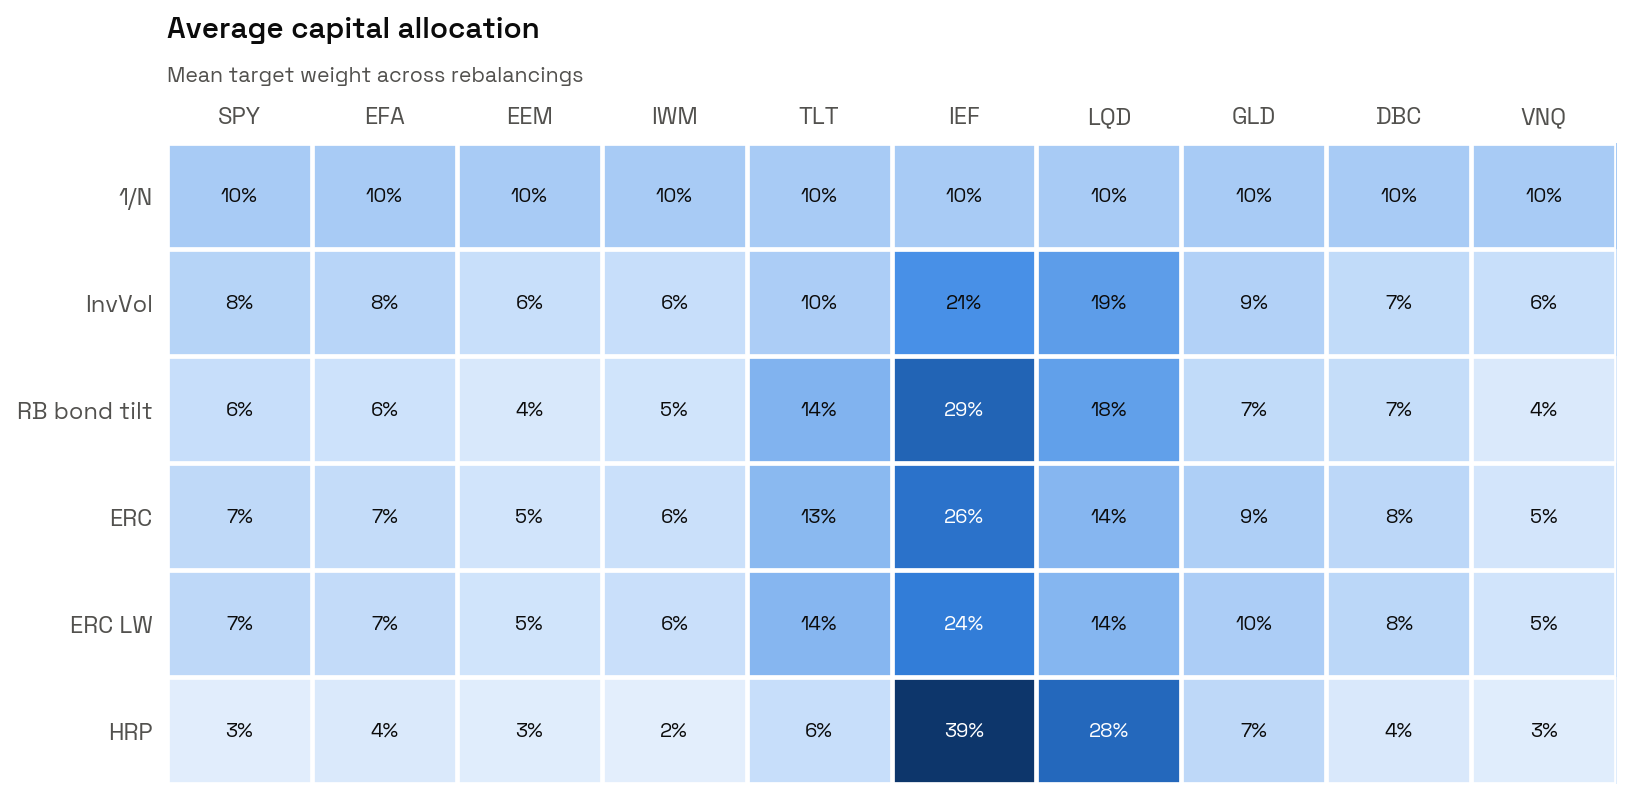
\includegraphics[width=\linewidth]{report_06_avg_weights.png}

\vspace{1cm}
{\sffamily\small
\begin{tabular}{@{}l@{\hspace{1.2cm}}l@{}}
\color{ink2}Auteur & Jean Philippe N'DRI \\
\color{ink2}Version & Septembre 2026 \\
\color{ink2}Code & \py{portopt/}
\end{tabular}}
\restoregeometry
\end{titlepage}

{\hypersetup{linkcolor=ink}\tableofcontents}
\thispagestyle{fancy}
\newpage

% =============================================================================
\section{Installation}\label{sec:install}

\py{portopt} demande Python 3.10 ou plus. Depuis la racine du dépôt :

\begin{shell}
pip install -e .              # numpy, pandas, scipy, yfinance
pip install -e ".[plot]"      # + matplotlib, pour le module plot
pip install -e ".[dev]"       # + matplotlib et pytest
pytest                        # 42 tests, quelques secondes
\end{shell}

Le dépôt est organisé ainsi :

\begin{pyout}
portopt/
  data.py          téléchargement, nettoyage, rendements, univers simulé
  estimator.py     règles d'allocation et estimateurs de covariance
  backtester.py    backtest walk-forward
  metric.py        indicateurs de performance et de risque
  plot.py          graphiques et rapport PNG
  fonts/           polices utilisées par plot (licence OFL)
examples/run_backtest.py   comparaison complète en ligne de commande
docs/                      méthodologie, ce guide, figures
tests/                     tests unitaires
\end{pyout}

Pour vérifier l'installation sans réseau :

\begin{python}
from portopt.data import simulate_returns
from portopt import ERC, run_backtests, summary

rets, _ = run_backtests(simulate_returns(), {"ERC": ERC()}, 252, 21)
print(summary(rets).loc["Sharpe"].round(3))
\end{python}
\begin{pyout}
ERC    0.776
Name: Sharpe, dtype: float64
\end{pyout}

% =============================================================================
\section{Conventions}\label{sec:conv}

La librairie repose sur quelques conventions. Les connaître évite la plupart des erreurs.

\begin{center}\small
\begin{tabularx}{\linewidth}{@{}l>{\raggedright\arraybackslash}X@{}}
\toprule
Objet & Convention \\
\midrule
Rendements & \py{DataFrame} indexé par un \py{DatetimeIndex} (dates en lignes), une colonne par actif. Rendements \textbf{simples}, pas logarithmiques. \\
Date & La ligne $t$ contient le rendement de la clôture $t-1$ à la clôture $t$. \\
Valeur manquante & \py{NaN} signifie « actif non disponible ». Le backtester n'investit que dans les actifs sans \py{NaN} sur la fenêtre d'estimation. \\
Poids & \py{pd.Series} indexée par actif, positive, de somme 1. \\
Fréquence & Quotidienne par défaut (\py{periods_per_year=252}). Pour d'autres fréquences, passer \py{periods_per_year} aux fonctions de \py{metric}. \\
Taux sans risque & \py{sharpe_ratio(rf=...)} : taux \textbf{annuel}. \\
Seuil du Sortino & \py{sortino_ratio(target=...)} : seuil \textbf{par période}. \\
Seuil du PSR & \py{probabilistic_sharpe_ratio(sr_benchmark=...)} : Sharpe \textbf{annualisé}. \\
Coûts & \py{transaction_cost_bps} en points de base, appliqués au turnover one-way. \\
\bottomrule
\end{tabularx}
\end{center}

% =============================================================================
\section{Module data}\label{sec:data}

\subsection{Obtenir des rendements}

\py{load_returns} enchaîne téléchargement, nettoyage et calcul des rendements :

\begin{python}
from portopt import load_returns

R = load_returns(["SPY", "TLT", "GLD"], start="2010-01-01", end="2024-12-31",
                 cache_dir="data_cache")
\end{python}

Avec \py{cache_dir}, le premier appel enregistre les prix en CSV et les appels suivants
les relisent sans réseau. Le nom du fichier dépend des tickers, des dates et du champ
demandé : changer un paramètre déclenche un nouveau téléchargement.

\begin{center}\small
\begin{tabularx}{\linewidth}{@{}l>{\raggedright\arraybackslash}X@{}}
\toprule
Fonction & Rôle et paramètres \\
\midrule
\py{download_prices} & Prix Yahoo Finance. \py{tickers}, \py{start}, \py{end} (exclue), \py{field="Close"}, \py{auto_adjust=True} (prix ajustés des dividendes et splits), \py{cache_dir}. \\
\py{clean_prices} & \py{ffill_limit=5} : comble les trous d'au plus 5 jours avec la dernière valeur. \py{min_history} : retire les actifs ayant moins d'observations. Jamais de remplissage avec une valeur future. \\
\py{compute_returns} & \py{method="simple"} ou \py{"log"}, \py{period=1}. Retire les premières lignes sans rendement. \\
\py{resample_returns} & Change de fréquence en composant les rendements : \py{rule="W-FRI"}, \py{"ME"}, etc. \\
\py{load_returns} & Les trois étapes ci-dessus, en rendements simples. \\
\py{simulate_returns} & Univers simulé de 10 ETF (SPY, EFA, EEM, IWM, TLT, IEF, LQD, GLD, DBC, VNQ) : \py{n_obs=3780}, \py{start}, \py{seed=15}. \\
\bottomrule
\end{tabularx}
\end{center}

\subsection{Travailler hors ligne}

\begin{python}
from portopt.data import simulate_returns

R = simulate_returns()
print(R.shape, R.index[0].date(), R.index[-1].date())
print(list(R.columns))
\end{python}
\begin{pyout}
(3780, 10) 2010-01-01 2024-06-27
['SPY', 'EFA', 'EEM', 'IWM', 'TLT', 'IEF', 'LQD', 'GLD', 'DBC', 'VNQ']
\end{pyout}

Le simulateur reproduit des corrélations réalistes, des régimes de stress et des queues
épaisses. Il sert aux tests, aux exemples et à la documentation.

\subsection{Nettoyer ses propres prix}

Si vous avez vos propres prix (fichier CSV, base interne), passez-les à
\py{clean_prices} puis \py{compute_returns}. L'exemple ci-dessous simule un actif coté
plus tard (SPY) et un trou de trois jours (EFA) :

\begin{python}
import numpy as np
from portopt.data import clean_prices, compute_returns

prices = 100 * (1 + R).cumprod()
prices.iloc[:300, 0] = np.nan         # SPY absent des 300 premières dates
prices.iloc[1000:1003, 1] = np.nan    # trou de 3 jours sur EFA

rets = compute_returns(clean_prices(prices))
print(rets.isna().sum().head(3))
\end{python}
\begin{pyout}
SPY    300
EFA      0
EEM      0
\end{pyout}

Le trou d'EFA est comblé ; les dates où SPY n'existait pas restent en \py{NaN}, et le
backtester n'investira dans SPY qu'une fois son historique complet.

\subsection{Changer de fréquence}

\begin{python}
from portopt.data import resample_returns

W = resample_returns(R, "W-FRI")   # hebdomadaire, fin de semaine le vendredi
M = resample_returns(R, "ME")      # mensuel, fin de mois
print(W.shape, M.shape)
\end{python}
\begin{pyout}
(757, 10) (174, 10)
\end{pyout}

\begin{attention}
En hebdomadaire ou en mensuel, pensez à passer \py{periods_per_year=52} ou \py{12} aux
fonctions de \py{metric} et à \py{annualized_turnover} (section~\ref{sec:freq}).
\end{attention}

% =============================================================================
\section{Module estimator}\label{sec:est}

\subsection{Interface commune}

Toutes les règles d'allocation suivent la même interface, inspirée de scikit-learn :

\begin{python}
import numpy as np
import pandas as pd
from portopt import ERC, risk_contributions

window = R.iloc[-252:]                        # une fenêtre d'un an
est = ERC(cov_method="ledoit_wolf").fit(window)
print(est.weights_.round(3))
\end{python}
\begin{pyout}
SPY    0.073
EFA    0.064
EEM    0.048
IWM    0.060
TLT    0.145
IEF    0.251
LQD    0.146
GLD    0.089
DBC    0.071
VNQ    0.054
Name: ERC, dtype: float64
\end{pyout}

\begin{python}
print(risk_contributions(est.weights_, est.cov_).round(3))
\end{python}
\begin{pyout}
[0.1 0.1 0.1 0.1 0.1 0.1 0.1 0.1 0.1 0.1]
\end{pyout}

\begin{center}\small
\begin{tabularx}{\linewidth}{@{}l>{\raggedright\arraybackslash}X@{}}
\toprule
Élément & Description \\
\midrule
\py{fit(returns)} & Calcule les poids sur une fenêtre sans \py{NaN} ; renvoie l'estimateur. \\
\py{weights_} & Poids (\py{pd.Series}, somme 1, positifs). Son nom est celui de la classe. \\
\py{cov_} & Covariance utilisée (\py{ndarray}), pour les règles qui en estiment une. \\
\py{name} & Nom de la classe, utilisé comme libellé par défaut. \\
\py{cov_method} & \py{"sample"}, \py{"ledoit_wolf"}, \py{"ewma"} ou une fonction \py{returns -> ndarray}. \\
\bottomrule
\end{tabularx}
\end{center}

\subsection{Règles disponibles}

\begin{center}\small
\begin{tabularx}{\linewidth}{@{}l>{\raggedright\arraybackslash}X@{}}
\toprule
Classe & Paramètres propres \\
\midrule
\py{EqualWeight()} & aucun ; $w_i=1/N$. \\
\py{InverseVolatility(exponent=1.0)} & $w_i\propto\sigma_i^{-k}$ ; \py{exponent=2} pour l'inverse variance. \\
\py{RiskParity(budgets=None, tol=1e-10, max_iter=10000)} & budgets de risque : \py{dict}, liste ou \py{pd.Series}, un par actif, strictement positifs, normalisés automatiquement. \py{None} donne l'ERC. Attribut \py{n_iter_}. \\
\py{ERC(tol, max_iter)} & \py{RiskParity} avec budgets égaux. \\
\py{HRP(linkage="single", split="bisection")} & \py{linkage} : \py{"single"}, \py{"complete"}, \py{"average"}, \py{"ward"} ; \py{split} : \py{"bisection"} (article original) ou \py{"dendrogram"}. Attributs \py{order_} et \py{linkage_matrix_}. \\
\bottomrule
\end{tabularx}
\end{center}

\subsection{Budgets de risque}

\begin{python}
from portopt import RiskParity

budgets = {t: 1 for t in R.columns} | {"TLT": 2, "IEF": 2, "LQD": 2}
rb = RiskParity(budgets=budgets).fit(window)
rc = risk_contributions(rb.weights_, rb.cov_)
print(pd.Series(rc, index=R.columns).round(3))
\end{python}
\begin{pyout}
SPY    0.077
EFA    0.077
EEM    0.077
IWM    0.077
TLT    0.154
IEF    0.154
LQD    0.154
GLD    0.077
DBC    0.077
VNQ    0.077
\end{pyout}

Les budgets $2$ et $1$ sont normalisés : les trois ETF obligataires portent chacun
$2/13\approx15.4\pct$ du risque. Un budget manquant pour un actif de la fenêtre lève
\py{ValueError: budgets missing for some assets of the window.}

\subsection{HRP}

\begin{python}
from portopt import HRP

h = HRP(linkage="ward", split="dendrogram").fit(window)
print(h.order_)
\end{python}
\begin{pyout}
['LQD', 'TLT', 'IEF', 'VNQ', 'SPY', 'IWM', 'EFA', 'EEM', 'GLD', 'DBC']
\end{pyout}

\py{order_} donne l'ordre des feuilles de l'arbre, et \py{linkage_matrix_} l'arbre
lui-même, que SciPy sait tracer :

\begin{python}
from scipy.cluster.hierarchy import dendrogram
dendrogram(h.linkage_matrix_, labels=list(window.columns))
\end{python}

\subsection{Choisir l'estimateur de covariance}

Toute règle accepte une fonction à la place d'un nom. Par exemple, une covariance
diagonale (corrélations ignorées) transforme l'ERC en inverse volatilité, ce qu'on peut
vérifier :

\begin{python}
from portopt import InverseVolatility

diag_cov = lambda r: np.diag(r.var().to_numpy())
w1 = ERC(cov_method=diag_cov).fit(window).weights_
w2 = InverseVolatility().fit(window).weights_
print(np.abs(w1 - w2).max())
\end{python}
\begin{pyout}
8.326672684688674e-17
\end{pyout}

Les estimateurs sont aussi disponibles directement :

\begin{python}
from portopt import estimate_cov, ledoit_wolf_cov
from portopt.estimator import ewma_cov

S = estimate_cov(window, "sample")
Sigma, delta = ledoit_wolf_cov(window)       # delta : intensité du shrinkage
S_ewma = ewma_cov(window, halflife=63)
\end{python}

\subsection{Écrire sa propre règle}

Il suffit d'hériter de \py{BaseEstimator} et d'implémenter \py{_compute_weights}, qui
reçoit une fenêtre sans \py{NaN} et renvoie un vecteur de poids. \py{fit} met à zéro les
poids négatifs et normalise la somme à 1. Exemple : le portefeuille de variance minimale
long-only.

\begin{python}
from scipy.optimize import minimize
from portopt import BaseEstimator

class MinVariance(BaseEstimator):
    def _compute_weights(self, returns):
        cov = self._cov(returns)             # applique cov_method
        cov = cov / np.trace(cov)            # mise à l'échelle, même solution
        n = cov.shape[0]
        res = minimize(lambda w: w @ cov @ w, np.full(n, 1 / n),
                       jac=lambda w: 2 * cov @ w, method="SLSQP",
                       bounds=[(0, 1)] * n,
                       constraints={"type": "eq", "fun": lambda w: w.sum() - 1},
                       options={"ftol": 1e-12, "maxiter": 500})
        return res.x

print(MinVariance(cov_method="ledoit_wolf").fit(window).weights_.round(3))
\end{python}
\begin{pyout}
SPY    0.130
EFA    0.020
EEM    0.000
IWM    0.014
TLT    0.000
IEF    0.611
LQD    0.155
GLD    0.020
DBC    0.051
VNQ    0.000
Name: MinVariance, dtype: float64
\end{pyout}

\begin{attention}
Sans la mise à l'échelle et le gradient explicite, SLSQP s'arrête dès le premier pas :
les variances quotidiennes sont de l'ordre de $10^{-5}$, et la fonction objectif passe
sous sa tolérance par défaut. L'optimiseur renvoie alors exactement 1/N, sans message
d'erreur. Normaliser la covariance ne change pas la solution.
\end{attention}

% =============================================================================
\section{Module backtester}\label{sec:bt}

\subsection{Un backtest}

\begin{python}
from portopt import Backtester

bt = Backtester(R, ERC(), in_sample=252, out_of_sample=21, transaction_cost_bps=5)
r = bt.run()
print(type(r).__name__, r.shape, r.index[0].date(), r.name)
\end{python}
\begin{pyout}
Series (3528,) 2010-12-21 ERC
\end{pyout}

Les rendements commencent après la première fenêtre de 252 dates. Chaque date de
rebalancement utilise uniquement les données antérieures.

\begin{center}\small
\begin{tabularx}{\linewidth}{@{}l>{\raggedright\arraybackslash}X@{}}
\toprule
Paramètre & Rôle \\
\midrule
\py{returns} & rendements (\py{DataFrame}), \py{NaN} autorisés. \\
\py{estimator} & règle d'allocation ; copiée à chaque rebalancement. \\
\py{in_sample} & longueur de la fenêtre d'estimation $L$ (au moins 2, et inférieure au nombre de dates). \\
\py{out_of_sample} & période de détention $H$ entre deux rebalancements. \\
\py{window} & \py{"rolling"} (fenêtre glissante de $L$ dates) ou \py{"expanding"} (depuis la première date). \\
\py{transaction_cost_bps} & coût proportionnel au turnover, en points de base. \\
\py{drift} & \py{True} : les poids dérivent avec les prix entre deux rebalancements (réaliste). \py{False} : rebalancement quotidien gratuit vers la cible. \\
\py{min_assets} & nombre minimal d'actifs éligibles pour rebalancer ; sinon le portefeuille précédent est conservé. \\
\bottomrule
\end{tabularx}
\end{center}

\subsection{Ce que renvoie le backtest}

\begin{python}
print(bt.weights_.iloc[:3, :4].round(3))
print(bt.turnover_.iloc[:3].round(3))
print(round(bt.annualized_turnover(), 3))
\end{python}
\begin{pyout}
              SPY    EFA    EEM    IWM
2010-12-21  0.079  0.074  0.057  0.066
2011-01-19  0.078  0.070  0.053  0.065
2011-02-17  0.073  0.072  0.055  0.062

2010-12-21    1.000
2011-01-19    0.037
2011-02-17    0.027

0.488
\end{pyout}

\begin{center}\small
\begin{tabularx}{\linewidth}{@{}l>{\raggedright\arraybackslash}X@{}}
\toprule
Élément & Description \\
\midrule
\py{run()} & lance le backtest et renvoie les rendements nets de coûts (\py{pd.Series}). \\
\py{returns_}, \py{gross_returns_} & rendements nets et bruts de coûts. \\
\py{weights_} & poids cibles à chaque rebalancement (\py{DataFrame} dates $\times$ actifs). \\
\py{turnover_} & turnover one-way à chaque rebalancement ; le premier vaut 1 (départ en cash). \\
\py{annualized_turnover(periods_per_year=252)} & turnover moyen par an, hors construction initiale. \\
\py{risk_contributions(cov_method="sample")} & contributions au risque ex ante à chaque rebalancement. \\
\bottomrule
\end{tabularx}
\end{center}

\subsection{Actifs cotés en cours de période}

Un actif dont la fenêtre contient des \py{NaN} reçoit un poids nul, puis entre dans le
portefeuille dès qu'il a $L$ dates complètes. Aucun traitement n'est à faire en amont :

\begin{python}
R2 = R.copy()
R2.iloc[:600, 0] = np.nan                      # SPY coté à partir de la date 600
bt2 = Backtester(R2, HRP(), 252, 21)
bt2.run()
print(bt2.weights_["SPY"].iloc[0], round(bt2.weights_["SPY"].iloc[-1], 3))
\end{python}
\begin{pyout}
0.0 0.02
\end{pyout}

Pendant la détention, un \py{NaN} est traité comme un rendement nul (prix figé).

\subsection{Comparer plusieurs règles}

\begin{python}
from portopt import EqualWeight, run_backtests, summary

rules = {"1/N": EqualWeight(), "ERC": ERC(), "HRP": HRP()}
rets, bts = run_backtests(R, rules, 252, 21, transaction_cost_bps=5)
print(rets.shape, list(rets.columns))
\end{python}
\begin{pyout}
(3528, 3) ['1/N', 'ERC', 'HRP']
\end{pyout}

\py{run_backtests} applique la même grille à chaque règle et renvoie les rendements
(\py{DataFrame}, une colonne par règle) et le dictionnaire des \py{Backtester}. Les
paramètres supplémentaires (\py{window}, \py{drift}, \dots) sont transmis à chaque
backtest.

\begin{attention}
Passez un \textbf{dictionnaire} \py{{libellé: estimateur}}. Une liste est acceptée, mais
les libellés sont alors les noms de classe : \py{[ERC(), ERC(cov_method="ledoit_wolf")]}
lève une erreur, car les deux s'appelleraient \py{ERC}.
\end{attention}

% =============================================================================
\section{Module metric}\label{sec:metric}

\subsection{Le tableau de synthèse}

\begin{python}
turnover = {k: b.annualized_turnover() for k, b in bts.items()}
print(summary(rets, turnover=turnover).round(3))
\end{python}
\begin{pyout}
                     1/N      ERC      HRP
CAGR               0.069    0.062    0.061
Ann. mean          0.074    0.063    0.062
Ann. vol           0.114    0.082    0.070
Sharpe             0.644    0.772    0.879
Sortino            0.925    1.140    1.329
Calmar             0.254    0.325    0.408
Max DD            -0.273   -0.190   -0.150
Max DD duration  923.000  760.000  426.000
VaR 95%            0.010    0.008    0.006
CVaR 95%           0.017    0.012    0.010
Skew               0.195    0.648    0.893
Excess kurt       13.689   16.898   16.310
Hit ratio          0.535    0.540    0.534
PSR(SR>0)          0.992    0.998    1.000
Ann. turnover      0.383    0.488    1.203
\end{pyout}

\py{summary(returns, rf=0.0, periods_per_year=252, alpha=0.05, turnover=None)} accepte
une \py{Series} ou un \py{DataFrame}. La durée du drawdown est en nombre de périodes ;
VaR et CVaR sont des pertes positives sur une période.

\subsection{Les fonctions}

Toutes acceptent une \py{Series} (renvoient un nombre) ou un \py{DataFrame} (renvoient
une \py{Series}, une valeur par colonne).

\begin{center}\small
\begin{tabularx}{\linewidth}{@{}l>{\raggedright\arraybackslash}X@{}}
\toprule
Fonction & Résultat \\
\midrule
\py{total_return}, \py{cagr} & rendement cumulé, taux annuel composé \\
\py{annualized_mean}, \py{annualized_volatility} & moyenne $\times P$, écart-type $\times\sqrt P$ \\
\py{sharpe_ratio(r, rf=0.0)} & Sharpe annualisé ; \py{rf} annuel \\
\py{sortino_ratio(r, target=0.0)} & Sortino annualisé ; \py{target} par période \\
\py{calmar_ratio} & CAGR divisé par la valeur absolue du drawdown maximal \\
\py{wealth_index}, \py{drawdown_series} & courbe de richesse, drawdown à chaque date \\
\py{max_drawdown}, \py{max_drawdown_duration} & drawdown maximal (négatif), durée sous l'eau \\
\py{value_at_risk(r, alpha=0.05)}, \py{conditional_value_at_risk} & VaR et CVaR historiques \\
\py{skewness}, \py{excess_kurtosis}, \py{hit_ratio} & asymétrie, kurtosis excédentaire, part de rendements positifs \\
\py{probabilistic_sharpe_ratio(r, sr_benchmark=0.0)} & probabilité que le vrai Sharpe dépasse le seuil (annualisé) \\
\bottomrule
\end{tabularx}
\end{center}

\begin{python}
from portopt import metric as M

x = rets["ERC"]
print(round(M.sharpe_ratio(x), 3), round(M.sharpe_ratio(x, rf=0.03), 3))
print(round(M.probabilistic_sharpe_ratio(x), 3),
      round(M.probabilistic_sharpe_ratio(x, sr_benchmark=0.5), 3))
\end{python}
\begin{pyout}
0.772 0.412
0.998 0.848
\end{pyout}

Avec un taux sans risque de 3\pct, le Sharpe d'ERC tombe de 0.77 à 0.41. La probabilité
que son vrai Sharpe dépasse 0.5 n'est que de 85\pct.

\subsection{Autres fréquences}\label{sec:freq}

\begin{python}
W = resample_returns(R, "W-FRI")
wr, wbts = run_backtests(W, {"ERC": ERC()}, in_sample=52, out_of_sample=4)
tbl = summary(wr, periods_per_year=52)
print(tbl.loc[["CAGR", "Ann. vol", "Sharpe"]].round(3))
print(round(wbts["ERC"].annualized_turnover(periods_per_year=52), 3))
\end{python}
\begin{pyout}
            ERC
CAGR      0.063
Ann. vol  0.083
Sharpe    0.783
0.74
\end{pyout}

\py{in_sample} et \py{out_of_sample} sont exprimés en nombre de périodes : 52 semaines et
4 semaines ici.

% =============================================================================
\section{Module plot}\label{sec:plot}

\subsection{Le rapport complet}

\begin{python}
from portopt import plot

paths = plot.save_report(rets, bts, "outputs/charts")
print([p.name for p in paths])
\end{python}
\begin{pyout}
['01_wealth.png', '02_drawdowns.png', '03_rolling_vol.png', '04_rolling_sharpe.png',
 '05_metrics.png', '06_avg_weights.png', '07_avg_risk_contrib.png',
 '08_weights_1_n.png', '08_weights_erc.png', '08_weights_hrp.png']
\end{pyout}

\py{save_report} produit sept graphiques de comparaison et un graphique de poids par
stratégie. Chaque stratégie garde la même couleur dans tous les graphiques.

\fig{report_02_drawdowns.png}{\py{plot_drawdowns} : un panneau par stratégie, drawdown
maximal annoté.}

\subsection{Les fonctions}

\begin{center}\small
\begin{tabularx}{\linewidth}{@{}l>{\raggedright\arraybackslash}X@{}}
\toprule
Fonction & Graphique \\
\midrule
\py{use_style()} & active le style (fond blanc, polices Space Grotesk) ; appelé par \py{save_report}. \\
\py{plot_wealth(rets, log=True)} & croissance de 1, avec la valeur finale au bout de chaque courbe. \\
\py{plot_drawdowns(rets)} & drawdowns, un panneau par stratégie. \\
\py{plot_rolling(rets, stat="vol", window=252)} & volatilité ou Sharpe (\py{stat="sharpe"}) glissants. \\
\py{plot_metrics(summary_df, metrics=None)} & barres horizontales, un panneau par indicateur. \\
\py{plot_heatmap(df, title)} & tableau coloré annoté (poids, contributions au risque). \\
\py{plot_weights_through_time(bt.weights_, title)} & poids de chaque actif à chaque rebalancement. \\
\py{plot_correlation(R, order=None)} & matrice de corrélation, dans l'ordre souhaité (par exemple \py{h.order_}). \\
\py{colors_for(names)} & couleur attribuée à chaque stratégie. \\
\bottomrule
\end{tabularx}
\end{center}

Chaque fonction renvoie un objet matplotlib (\py{Axes} ou \py{Figure}) que l'on peut
modifier puis enregistrer :

\begin{python}
plot.use_style()
ax = plot.plot_wealth(rets)
ax.figure.savefig("wealth.png")
\end{python}

\begin{attention}
\py{plot_rolling} et \py{save_report} supposent des données quotidiennes (annualisation
sur 252 périodes). Pour des données hebdomadaires ou mensuelles, calculez les indicateurs
avec \py{summary(..., periods_per_year=...)} et utilisez les autres fonctions de tracé.
\end{attention}

% =============================================================================
\section{Recettes}\label{sec:recipes}

\subsection{Comparaison complète en ligne de commande}

\begin{shell}
python examples/run_backtest.py              # 10 ETF, Yahoo Finance, depuis 2008
python examples/run_backtest.py --synthetic  # univers simulé, sans réseau
python examples/run_backtest.py --in-sample 504 --out-of-sample 63 \
                                --tc-bps 10
\end{shell}

Le script compare six règles (1/N, InvVol, risk budgeting orienté obligations, ERC,
ERC Ledoit-Wolf, HRP) et écrit dans \py{outputs/} : \py{summary.csv},
\py{oos_returns.csv} et le rapport graphique dans \py{outputs/charts/}. Options :
\py{--start}, \py{--end}, \py{--in-sample}, \py{--out-of-sample}, \py{--tc-bps},
\py{--out}.

\subsection{Tester la robustesse aux paramètres}

La fenêtre $L$ et la période de détention $H$ sont des choix arbitraires. Un résultat
fiable doit résister à leur variation : on regarde le classement des règles sur une
grille, pas le meilleur couple.

\begin{python}
grid = {}
for L in (126, 252, 504):
    for H in (5, 21, 63):
        out, _ = run_backtests(R, rules, L, H, transaction_cost_bps=5)
        grid[(L, H)] = summary(out).loc["Sharpe"].rank(ascending=False).astype(int)
print(pd.DataFrame(grid).T)
\end{python}
\begin{pyout}
        1/N  ERC  HRP
126 5     3    2    1
    21    3    2    1
    63    3    2    1
252 5     3    2    1
    21    3    2    1
    63    3    2    1
504 5     3    1    2
    21    3    1    2
    63    3    2    1
\end{pyout}

1/N est dernier partout ; l'ordre entre ERC et HRP dépend de la fenêtre.

\subsection{Mesurer la part de hasard du calendrier}

Décaler la date de départ change les dates de rebalancement. L'écart obtenu mesure ce
qui relève du hasard du calendrier (\emph{timing luck}) :

\begin{python}
luck = {}
for offset in range(0, 21, 5):
    out, _ = run_backtests(R.iloc[offset:], {"ERC": ERC()}, 252, 21)
    luck[offset] = summary(out).loc["Sharpe", "ERC"]
print(pd.Series(luck).round(3))
\end{python}
\begin{pyout}
0     0.776
5     0.787
10    0.782
15    0.777
20    0.782
\end{pyout}

Ici l'écart est faible (0.78 $\pm$ 0.01) : le résultat d'ERC ne dépend pas du calendrier.

\subsection{Exporter les résultats}

\begin{python}
rets.to_csv("oos_returns.csv")
summary(rets).to_csv("summary.csv")
bts["ERC"].weights_.to_csv("erc_weights.csv")
bts["ERC"].risk_contributions().to_csv("erc_risk_contrib.csv")
\end{python}

\subsection{Régénérer la documentation}

\begin{shell}
python docs/make_figures.py                     # figures de la méthodologie
cd docs && latexmk -xelatex methodology.tex     # méthodologie (FR)
latexmk -xelatex methodology_en.tex             # méthodologie (EN)
latexmk -xelatex user_guide.tex                 # ce guide
\end{shell}

% =============================================================================
\section{Erreurs fréquentes}\label{sec:faq}

\begin{center}\small
\begin{longtable}{@{}>{\raggedright}p{5.2cm}>{\raggedright\arraybackslash}p{9.6cm}@{}}
\toprule
Message & Cause et solution \\
\midrule
\endhead
\py{returns contain NaN: select a clean universe before fitting.} & \py{fit} appelé directement sur une fenêtre avec des \py{NaN}. Sélectionner les actifs complets (\py{window.dropna(axis=1)}) ou passer par le \py{Backtester}, qui le fait seul. \\
\py{budgets missing for some assets of the window.} & \py{RiskParity} : un actif de la fenêtre n'a pas de budget. Donner un budget à chaque actif. \\
\py{budgets must be strictly positive (log barrier).} & Budget nul ou négatif. Pour exclure un actif, le retirer des rendements. \\
\py{in_sample (...) >= number of observations (...).} & Fenêtre plus longue que l'historique. Réduire \py{in_sample} ou allonger l'historique. \\
\py{call run() first.} & \py{annualized_turnover()} ou \py{risk_contributions()} avant \py{run()}. \\
\py{Several estimators share the name [...]} & Liste passée à \py{run_backtests} avec deux règles de même classe. Utiliser un dictionnaire. \\
\py{No data returned by Yahoo Finance for [...]} & Pas de réseau, ticker inconnu ou période vide. Vérifier les tickers ; travailler avec \py{cache_dir} ou \py{simulate_returns()}. \\
\py{No data for tickers: [...]} & Certains tickers n'ont renvoyé aucun prix. Les retirer de la liste. \\
\py{Field '...' not in [...]} & Champ absent : avec \py{auto_adjust=True}, Yahoo ne renvoie plus \py{Adj Close} ; utiliser \py{field="Close"}, déjà ajusté. \\
Poids d'une règle personnalisée égaux à 1/N & Optimiseur arrêté dès le départ à cause de l'échelle des variances (section~\ref{sec:est}). Normaliser la covariance et fournir le gradient. \\
Indicateurs aberrants en hebdomadaire & \py{periods_per_year} laissé à 252. Passer 52 (ou 12 en mensuel). \\
\bottomrule
\end{longtable}
\end{center}

% =============================================================================
\section{Référence de l'API}\label{sec:api}

\subsubsection*{portopt.data}
\begin{pyout}
download_prices(tickers, start=None, end=None, field="Close", auto_adjust=True,
                cache_dir=None) -> DataFrame
clean_prices(prices, ffill_limit=5, min_history=None) -> DataFrame
compute_returns(prices, method="simple", period=1) -> DataFrame | Series
resample_returns(returns, rule="W-FRI", method="simple") -> DataFrame | Series
load_returns(tickers, start=None, end=None, method="simple", cache_dir=None,
             ffill_limit=5) -> DataFrame
simulate_returns(n_obs=3780, start="2010-01-01", seed=15) -> DataFrame
\end{pyout}

\subsubsection*{portopt.estimator}
\begin{pyout}
EqualWeight(cov_method="sample")
InverseVolatility(cov_method="sample", exponent=1.0)
RiskParity(cov_method="sample", budgets=None, tol=1e-10, max_iter=10000)
ERC(cov_method="sample", tol=1e-10, max_iter=10000)
HRP(cov_method="sample", linkage="single", split="bisection")
BaseEstimator.fit(returns) -> self      # attributs weights_, cov_
estimate_cov(returns, method="sample") -> ndarray
sample_cov(returns) -> ndarray
ledoit_wolf_cov(returns) -> (ndarray, float)
ewma_cov(returns, halflife=63.0) -> ndarray
risk_contributions(weights, cov) -> ndarray
\end{pyout}

\subsubsection*{portopt.backtester}
\begin{pyout}
Backtester(returns, estimator, in_sample, out_of_sample, window="rolling",
           transaction_cost_bps=0.0, drift=True, min_assets=1)
  .run() -> Series
  .annualized_turnover(periods_per_year=252) -> float
  .risk_contributions(cov_method="sample") -> DataFrame
run_backtests(returns, estimators, in_sample, out_of_sample, **kwargs)
  -> (DataFrame, dict[str, Backtester])
\end{pyout}

\subsubsection*{portopt.metric}
\begin{pyout}
summary(returns, rf=0.0, periods_per_year=252, alpha=0.05, turnover=None) -> DataFrame
total_return(r)
cagr(r, periods_per_year=252)
annualized_mean(r, periods_per_year=252)
annualized_volatility(r, periods_per_year=252)
sharpe_ratio(r, rf=0.0, periods_per_year=252)
sortino_ratio(r, target=0.0, periods_per_year=252)
calmar_ratio(r, periods_per_year=252)
wealth_index(r, start=1.0)
drawdown_series(r)
max_drawdown(r)
max_drawdown_duration(r)
value_at_risk(r, alpha=0.05)
conditional_value_at_risk(r, alpha=0.05)
skewness(r)
excess_kurtosis(r)
hit_ratio(r)
probabilistic_sharpe_ratio(r, sr_benchmark=0.0, periods_per_year=252)
\end{pyout}

\subsubsection*{portopt.plot}
\begin{pyout}
use_style()   colors_for(names)
plot_wealth(returns, ax=None, log=True, colors=None, title="Growth of 1")
plot_drawdowns(returns, colors=None, ncols=3)
plot_rolling(returns, stat="vol", window=252, colors=None, ax=None)
plot_metrics(summary, metrics=None, colors=None, ncols=3)
plot_heatmap(values, title, subtitle="", fmt="{:.0%}", diverging=False, ax=None,
             vmax=None, annot_size=8.5)
plot_weights_through_time(weights, title, ax=None)
plot_correlation(returns, order=None, title="Correlation matrix", subtitle="", ax=None)
save_report(returns, backtesters, out_dir, rolling_window=252) -> list[Path]
\end{pyout}

\end{document}
